\begin{savequote}[75mm]
Either the rest of the world can't live like the developed world or we need, as a society, to think more about the technology of providing these services with less intensive use of at least certain  resources. We need to do a more diligent job of good housekeeping.
\qauthor{Thomas E. Graedel (1940- )}
\end{savequote}

\chapter{Quantifying Energy-Water Resource Usage}
\label{Chapter 3}

\newpage

\section{Quantifying Life-Cycle Energy-Water Resource Usage Efficiency}

The third principle challenge which must be overcome in the pursuit of this dissertation's stated research objective is the development of a systematic method for quantifying the life-cycle energy-water resource utilization efficiency of water reuse systems involving significant artificial groundwater recharge components. For this purpose, the author decided it prudent to build upon a substantial body of previous research in this area by utilizing an existing life-cycle inventory (LCI) database comprising energy and material process flow data collected from a large sample of existing WWTP operations and reuse facilities. The novelty of this approach lay in the dynamic parameterization of these models for a given study via the integration with the two previous modeling components related to (1) determining the suitable sites for recharge infrastructure and (2) determining the optimal corridors for the distribution network supplying the treated wastewater from the WWTP. As it shall be shown, taking the effort to correctly parameterize this model using contextual geographic information goes a long way towards improving both the accuracy and the precision of the model's outputs.

\section{Life Cycle Assessment and Inventory Modeling}

Life-cycle assessment (LCA) is an environmental accounting framework that was developed to systematically quantify the material and energy inputs and outputs from a product, process, or system throughout all its stages of life. It uses a cradle-to-grave or, in some cases, cradle-to-cradle perspective, to evaluate the design processes as well as the entire supply chain associated with manufacturing, transportation, the use phase, and waste management \cite(Rebitzer2004). Practically, process based LCA analyses, which shall be the focus of the remainder of this discussion, incorporate two distinct modeling phases. The first involves the development of a Life-cycle Inventory model is a cumulative record of all of the materials and energy flows required to deliver a single functional unit of the product or process in question. The second, optional, phase of LCA analyses is the Life-cycle Impact Assessment (LCIA) component. An LCIA model attempts to translate the raw energy and material flows contained within the LCI into different categories of environmental impacts such as global warming potential, ocean acidification, freshwater eutrophication, etc. 

In the context of this discussion, one of the stated goals of this dissertation project was to quantify the energy-water usage efficiency of artificial groundwater recharge projects involving the reuse of treated municipal wastewater. In order to accomplish this goal custom LCI models will be developed for five case study regions in which the distribution networks responsible for transporting the treated wastewater for its point of origin, the WWTP, to its destination point of consumption, an artificial groundwater infiltration basin positioned at a designated destination location, upstream within the regional watershed. The raw data supporting the creation of each of these custom LCI models shall be derived from the UC Berkeley supported Web Water-Energy Sustainability Tool (WWEST). In each case study, the scope of this LCI modeling exercise shall be limited to the construction and operational requirements associated with the WWTP plant, the treated water distribution network, and the infiltration basin. This system boundary has been defined in such a way as to emphasize the dynamic contribution of the treated wastewater distribution to the LCI of a given functional unit of treated wastewater delivered to the sub-surface in the face of variable geographic context.

\section{Wastewater Treatment Processes}

The phrase wastewater treatment encompasses a wide variety of different processes and operational facilities depending upon: the quality of the influent water, the volume of the influent water, and the desired quality/end-use application for the treated effluent water. In the United States the operation of WWTPs are regulated at both the State and Federal levels. At the Federal level the principle regulatory agency is the United States Environmental Protection Agency (USEPA) and the principle regulatory program is the National Pollutant Discharge Elimination System (NPDES). According to the legal mandate of the NPDES, WWTP operators (as well as a wide variety of other entities) are required to apply, at regular time intervals, for discharge permits which provide them with the legal right to release waters containing limited concentrations of regulated pollutants into the environment. Also under this mandate, the USEPA is required to distribute these permits and enforce non-compliance with their terms.

Since the inception of the NPDES program, the USEPA has worked to make readily accessibly a centralized database of all registered permit holders within the United States. This database in interesting for the purposes of this project in that it contains spatially referenced information about the operational aspects of every operating WWTP in the U.S. Crucially, this information includes data on maximum daily permitted flow rates and total maximum daily loads that can be used to parameterize the type of process based LCI model facilitated by the WWEST tool.

In terms of their basic physical layout and operational requirements, WWTPs are typically constructed with a tiered layout; comprising primary treatment, secondary treatment, and sometimes, various so called tertiary processes. Both primary and secondary treatment are terms that come with narrow legal definitions and are implemented at nearly all WWTP plants handling municipal sewage discharges. Tertiary treatment processes are more loosely defined and encompass a suite of advanced treatment processes that are so costly that they tend to only be implemented at a minority of WWTP that are subject to a unique  circumstances in terms of influent pollutant loadings/composition or requirements associated with designed high purity effluent end-use applications.

Primary treatment encompasses processes and equipment dedicated to the physical separation of non-soluble waste constituents present in the influent wastewater stream. Within a WWTP, a number of distinct processes are often lumped together as being part of the primary treatment. For example, when water first enters the WWTP it is guided through a series of progressively refined grates to screen out bulk pollutants such as anthropogenic trash or natural plant and animal detritus. Following from this bulk screening phase, the water is guided into a series of settling basins where its movement is slowed to crawl to facilitate the settlement of suspended pollutant materials such as sediment. Due to the slow rate at which this settling process proceeds, the physical infrastructure which supports it can comprise a significant fraction of the overall footprint of a WWTP; particularly for those with high flow volume processing requirements.

Secondary treatment encompasses processes and equipment dedicated to the biological (and sometimes chemical) degradation of soluble waste constitutes present in the influent wastewater stream. In most municipal WWTP secondary treatment is accomplished through a passively aspirated, aerobic biological digestion reactors. In these reactors large colonies of bacterial species are cultivated on high surface area media using the organic components of the influent wastewater stream as a feedstock for the continued growth. At the end of their life cycle, the bacteria fall to base of the reactor tank and must be continuously removed in the form of a product known as activated sludge.

Tertiary treatment encompasses processes and equipment dedicated to the removal of soluble inorganic and some organic chemical species (including some viruses and pharmaceutical agents) present within the influent wastewater stream. At present, tertiary treatment processes are not mandatory for all WWTP facilities regulated under the NPDES program. In general, they tend to only be implemented at those specific locations in which a last and credible threat to public or environmental health has been identified and for which a targeted tertiary treatment process exists to address. In this way, mandates for tertiary treatment are typically instigated at the state or local level and done so on a case by case basis. Among the most common tertiary treatment processes include: reverse osmosis filtration, batch irradiation with ultra-violent light, the application of specialized chemical amendments, de-nitrification processes, and others.

For the purposes of this analysis and the customized LCI models which shall be constructed as part of the case study investigations, only primary and secondary treatment processes shall be included in the scope. This decision has been made to eliminate a substantial bias in the inventory models process flows that might be associated with a single specialized tertiary treatment procedure.  

\section{Water Distribution Infrastructure}

The immediate delivery and reuse of treated wastewater for various municipal and agricultural end-use applications is still a relatively new phenomenon. As such, the regulatory landscape surrounding such practices is still not well defined at the Federal level here in the United States. Consequently, what regulations due exist, typically have been enacted at the State and local levels, with the most advanced frameworks, unsurprisingly, existing in those states such as Florida, California, and Arizona where the popularity of reuse as viable alternative source of freshwater supply, has been surging in recent years.

In all of the locations within the United States for which solid regulatory frameworks surrounding reuse currently exist, there are strong constraints governing the use of existing water distribution infrastructure for the transportation of treated wastewater from its point of origin, the WWTP, to its point of end-use. These regulations, without exception, stipulate that treated wastewater, even if returned to a level of quality consistent with requirements for potable use, cannot be conveyed using existing distribution infrastructure carrying potable water for human consumption in municipal areas. Due to this regulatory constraint, all treated wastewater destined for some sort of municipal reuse must be carried through dedicated parallel distribution infrastructure. In California, this infrastructure is easily identified at locations where treated wastewater is being reused due to the bright purple color of all the pipes. This color encoding is meant to be a strong visual reminder that the water being carried within them has not been deemed, from a regulatory perspective, as being fit for direct human consumption. 

The requirement that treated wastewater, regardless of its standard of treatment and anticipated end use application, be transported using a separate parallel distribution network is expected to be a crucial factor in determining the overall life-cycle energy-water usage efficiency of large scale water reuse systems feeding into artificial groundwater recharge basins. The reasoning behind this expectation is based upon the interaction of the following two key factors. [1] Water is a dense material, and thus it is very energy intensive to transport it over long distances and against steep elevation gradients. [2] Artificial groundwater recharge basins typically require fairly large amounts of contiguous land area that are situated in fairly close proximity to highly developed urban and suburban communities. Municipal water resource management agencies are tightly constrained in terms of the operating budgets from which they are able to draw funds to procure new land holdings for the purpose of constructing artificial recharge basins. Thus, artificial recharge basins , primarily to economic constraints, are typically located fairly far afield from the WWTPs which feed them.
 
\section{WWEST Recycled Water Reuse Life Cycle Inventory Model}

The WWEST Recycled Water Reuse Life-cycle Inventory Model refers to an integrated life-cycle inventory database and modeling framework for understanding the environmental impacts of wastewater treatment and reuse processes that was developed by a team of academic researchers operating out of the University of California at Berkeley College of Engineering. The principal investigator behind the project is Dr. Arpad Horvath, Professor of Civil and Environmental Engineering, and a specialist in the environmental impact assessment of civil infrastructure systems. The lead researcher on the WWEST project is Dr. Jennifer Stokes, with the initial development work on the WWEST model being completed as part of her doctoral dissertation project.

The LCI database underlying the WWEST toolset contains process flow information for the manufacture and operation of equipment and facilities involved in the supply, treatment, and distribution of municipal wastewater for the purpose of non-potable reuse. \ref{fig:WWESTsystem} 
provides a schematic overview of the WWEST database model components and their respective input data sources.

    \begin{figure}[!h]
        \begin{center}
        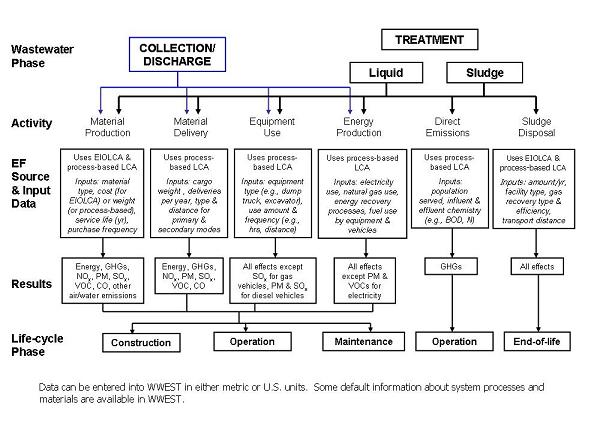
\includegraphics[width=5.5in]{figures/WWEST_System_Boundaries.jpg}
        \caption{WWEST Model System Boundaries}
        \label{fig:WWESTsystem}
        \end{center}
    \end{figure}
    
The WWEST LCI database can be accessed in two ways. The first, which provides full access to all of the attribute fields contained within the database, is via an excel spreadsheet that has been distributed with a built-in set of computational macros. The second method exposes a more limited range of the data values contained within the database and is accessible via a streamlined web application, also known as WWESTweb. The principle difference between the WWEST excel model and the web application is in the extent to which each allows the user to customize the various parameters associated with a hypothetic water reuse project and its supporting infrastructure. In this sense, the excel based model is more appropriate for building an LCI model to quantify the process flows attributable to an existing facility or which is in a very advanced stage of design planning. Conversely, the WWESTweb framework is more appropriate for less well defined scenario based planning exercises, where the primary goal is to assess the relative impact of major system design alternatives that have only roughly been fleshed out.

\section{Parameterizing Pump Energy Requirements} 

The WWEST model requires a number of key input parameters to be supplied by the user before it can be run. These parameters correspond to various attributes of the proposed reuse system including: pipe length and material information derived from the distribution network topology, estimates of distribution process energy consumption figures, and process based chemical inputs associated with any required tertiary treatment phases.

In order to facilitate the systematic parameterization of the WWEST model a programmatic workflow was developed which automates the calculation of a number of parameters from two input data sources: (1) the topology of the distribution network (i.e. the corridor solution from the MOGADOR optimization model) and (2) the expected daily flow rate derived from the maximum permitted flow value assigned to each WWTP facility through the NPDES permitting program. 

To illustrate how this workflow functions, take for example the process of calculating the expected energy requirements associated with the distribution of the treated wastewater from its source at that WWTP to its destination at the reuse facility. Estimating the instantaneous power output associated with the operation of a pipeline based water distribution system begins with Equation \ref{eq:pumpEnergy}.

      \begin{equation}
          P = \frac{Q * H_t * g * \rho}{E}
          \label{eq:pumpEnergy}
      \end{equation}
      
       \noindent \textit{Where:} \hfill

       \begin{center}
           $P = $ The instantaneous pump energy $(W)$ \\
           $Q = $ The instantaneous flow rate $(m^{3}/s)$\\
           $H_{t} = $ The total head $(m)$ \\
           $g = $ The gravitational constant $(m/s^{2})$ \\
           $\rho = $ The density of the fluid $(Kg/m^3)$ \\
           $E = $ The pump efficiency factor $(unitless)$ \\
       \end{center}

The first term in this expression $(Q)$, the instantaneous flow rate, can be computed by dividing the annual volume of processes by the WWTP by the number of seconds in a year. The second term $(H_t)$, the total system head, can be computed summing the individual static and dynamic head components as in the following Equations \ref{eq:staticHead} and \ref{eq:dynamicHead}. The last three terms $(g,\rho, \& E)$ are constants that are characteristic to the system.

       \begin{equation}
          H_s = e_{i} - e_{o}  
          \label{eq:staticHead}
       \end{equation}
      
       \noindent \textit{Where:} \hfill

       \begin{center}
           $H_s = $ The static head component \\
           $e_i = $ The elevation at pipeline inlet \\
           $e_o = $ The levation at pipeline output \\
       \end{center}

Equation \ref{eq:staticHead} describes how the static head can be computed as the difference between the elevations at the inlet and the outlet locations for the pipeline. When the corridor specification is known, this difference can be straightforwardly assessed by referencing the first and last subscript indices of the corridor to a raster based digital elevation model.

Computing the dynamic component $(H_d)$ of the total system head is a significantly more complicated process; however, it can, nonetheless, be similarly automated from the same detailed knowledge regarding the pipeline corridor specification and its underlying elevation profile. Equations \ref{eq:dynamicHead} through \ref{eq:frictionCoefficient} illustrate the sequence of operations by which dynamic head $(H_d)$ can be computed. 

       \begin{equation}
          H_d = \frac{K_{t} * V^2}{2g}
          \label{eq:dynamicHead}
       \end{equation}
       
       \noindent \textit{Where:} \hfill
       
       \begin{center}
           $H_d = $ The dynamic head component \\
           $K_t = $ The total system losses \\
           $V = $ The flow velocity \\
       \end{center}
       
The dynamic head term is a representation of the frictional forces that arise from the movement of water through the pipeline. These cumulative effective of these forces are represented by the term $(K_t)$, total losses, and are multiplied by the square of the velocity at which the water is flowing. The $(K_t)$ can be parsed into two separate components, $(K_p \& K_f)$, as shown in Equation \ref{eq:totalLosses}. These two terms represent the relative contribution of the friction associated with the movement of water over the textured surface of the pipeline interior walls and the friction associated with the movement of water through a tortuous pipeline that has various connective fittings such as elbow joints and flow control valves. 

       \begin{equation}
           K_{t} = K_{p} + K_{f}
           \label{eq:totalLosses}
       \end{equation}
       
       \noindent \textit{Where:} \hfill
       
       \begin{center}
           $K_p = $ The pipe loss component $(unitless)$ \\
           $K_f = $ The fitting loss component $(unitless)$ \\
       \end{center}       
       
Typically, the velocity term $(V)$ is computed from the product of a specific flow rate $(Q)$ and pipeline cross sectional area $(A)$ as in Equation \ref{eq:velocity}. However, in the case of this analysis, the pipeline cross sectional area was solved for by specifying a maximum permissible flow velocity $V_{max} = (10 m/s)$ relative to some designated flow rate.
       
       \begin{equation}
           V = \frac{Q}{A}
           \label{eq:velocity}
       \end{equation}
       
       \noindent \textit{Where:} \hfill
       
       \begin{center}
           $A = $ The cross sectional area of the pipe $(m^2)$\\
       \end{center}      
       
The component of the total losses attributable to the cumulative friction encounter along the pipeline's pipe section walls $(K_p)$ can be calculated from Equation \ref{eq:pipeLosses} as the product of a friction coefficient $(f)$ and the pipeline length $(L)$ divided by the diameter of the pipeline pipe sections $(D)$.
       
       \begin{equation}
           K_{p} = \frac{f * L}{D}
           \label{eq:pipeLosses}
       \end{equation}
       
       \noindent \textit{Where:} \hfill
       
       \begin{center}
           $f = $ The friction coefficient of the pipe $(unitless)$ \\
           $L = $ The cumulative length of all the pipe sections $(m)$ \\
           $D = $ The diameter of each pipe section $(m)$ \\
       \end{center}   
       
The friction component $(f)$ of the pipeline loss term $(K_p)$ can be computed from the empirically derived Equation \ref{eq:frictionCoefficient} where $(k)$ is a roughness factor that is characteristic to the pipe section material construction and $(Re)$ is the Reynolds number which is a dimensionless quantity that this associated to the smoothness with which a fluid flows and can be derived from the fluid's characteristic kinematic viscosity $(\upsilon)$ as in Equation \ref{eq:reynolds}.
       
       \begin{equation}
           f = \frac{0.25}{ \left\{ \log_{10}{ \frac{k}{3.75 * D} + \frac{5.74}{Re^{0.9}} } \right\}^{2} }
           \label{eq:frictionCoefficient}
       \end{equation}
       
       \noindent \textit{Where:} \hfill
       
       \begin{center}
           $k = $ The roughness factor of the pipe material $(m)$ \\
           $Re = $ The Reynolds Number of the fluid $(unitless)$ \\
       \end{center}   
       
       \begin{equation}
           Re = \frac{V * D}{\upsilon}
           \label{eq:reynolds}
       \end{equation}
       
       \noindent \textit{Where:} \hfill
       
       \begin{center}
           $\upsilon = $ The kinematic viscosity of the fluid $(m^2/s)$ \\
       \end{center}   
       
The fitting losses $(K_f)$, which makes up the second component of the total losses expression $(K_t)$ and which ultimately feeds into the calculation of dynamic head $(H_d)$, can be computed by using the corridor specification to cumulatively assess the need for various fitting components to facilitate pipeline deviations and flow control systems. The contribution of each fitting component to the total $(K_f)$ factor is empirically defined and can be iterative summing the contribution of each fitting $(K_n)$, multiplied by its appropriate fitting loss factor $(K'_n)$, along the entire length of the pipeline corridor as in Equation \ref{eq:fittingLossComponents}.

        \begin{equation}
            K_f = \sum\limits_{i=1}^n \left\{ (K_1 * K'_1) + \dots + (K_n * K'_n) \right\}
            \label{eq:fittingLossComponents}
        \end{equation}
    
       \noindent \textit{Where:} \hfill
       
       \begin{center}
           $K_n = $ The individual fitting loss component $(unitless)$ \\
           $K'_n = $ The individual fitting loss factor $(unitless)$ \\
       \end{center}
       
\section{Parameterizing Construction Material Requirements}

Once the pump energy associated with the corridor specification has been computed according to method laid out in Equations \ref{eq:pumpEnergy} - \ref{eq:fittingLossComponents} the next step is to estimate the volume of reinforced concrete that must be poured to facilitate the construction of the requisite infrastructural components of the proposed reuse system. It is assumed for the purpose of this analysis that these new infrastructural components will principally be associated with the need to install one or more pumping houses which will be situated along the length of the corridor. The determination of the size of each of these facilities and their concomitant material footprints will be determined on the basis of the total pump energy required for each corridor and the structure of the different elevation profiles. Consideration will be given to economies of scale in terms of the efficiency that can be achieved through the operation of larger pump systems.  
       
\section{Parameterizing Chemical Consumption Rates} 

The third key set of parameters that must be provided to the WWEST model are the volumes of any consumable chemical substances that must be provided to facilitate the tertiary treatment processes associated with the proposed reuse system. Ideally, the determination of these parameters would be made on the basis of the relative quality of the influent wastewater to that of the effluent treated water. However, the data requirements for this level of specificity in the model parameterization are significant and thus were left outside the scope of this analysis. As a result, all of the input parameter settings for the chemical consumption rates of the tertiary treatment processes were set to be equal to average values in the literature for a standard suite of treatment processes. These parameter settings can be found in the Parameter input tables contained within Appendix \ref{appendixA}.

\section{Estimating Net Water Usage Efficiency}

The final step towards the research program's overarching goal of estimating the life-cycle energy-water usage efficiency of proposed new reuse systems involves converting life-cycle energy consumption into predicted water consumption. This conversion can be accomplished by applying known water usage efficiency factors for a suite of energy generation technologies to the local grid mix responsible for producing the energy that will be supplied to the reuse system over its life-cycle. For the purpose of this analysis, the calculated metric will focus on the consumptive use of water for energy production as opposed to the non-consumptive use. This designation is important as the difference between the consumptive and non-consumptive water use profiles for a number of energy generation, and in particular, cooling technologies, can be non-trivial.

While the distribution of energy generation technologies is known from published statistics on the local grid mix associated with each of the five case study regions, a more granular breakdown of the precise thermoelectric cooling technology used by each category of energy producer is not known. In the absence of this detailed information a range of energy usage efficiencies -- corresponding to the min-max range of cooling technology efficiencies for each production method -- will be generated by the analysis, providing bounds to our uncertainty in the final calculated values. 

\section{Outputs of the WWEST Based Calculation}

The final output of the WWEST based calculation will involve three numbers. The first corresponds to the volume of wastewater that is to be treated and recycled by the proposed reuse operation over the course of a given year. The second corresponds to the life-cycle energy requirements attributable to this volume of water reuse each year at the site in question. The third number will be the quantity of water that must be consumed in order to generate the energy associated with the system's annualized life-cycle energy requirements. By computing the ratio of the second number to the third we will thus be left with an estimated ratio depicting the life-cycle energy-water usage efficiency of the proposed reuse system. If this ratio is greater than one it means that the proposed system is highly efficient, with more water being saved within the local basin each year than is consumed -- likely elsewhere, outside the basin -- to produce the energy associated with its operation. Similarly, if this ratio is greater than zero but less than one, the system is only partly efficient. And finally, if this ratio is less than zero, the system is highly inefficient, with more water being expended to the produce the energy required for the reuse operation that is saved by the operation of the reuse system. This third condition would essentially amount to a situation where water was being virtually imported into the basin in the form of the energy consumed by the reuse system.

\clearpage
